% Eigenvalue DOF sweep for the Coffey--Evans problem \texttt{coffey\_evans}: the eigenvalue index $k$
% against $\lambda_k$, at several DOF levels per method, over the
% \texttt{MATSLISE} reference. Indices 1 to 500.
% The methods are split over two panels, both repeating the reference.
%
% Requires in the preamble:
%   \usepackage{graphicx}
%   \usepackage{subfig}
%   \usepackage{epstopdf}   % the figures are EPS; needed under pdflatex,
%                           % which then wants -shell-escape. Not needed for
%                           % latex/dvips, which reads EPS directly.
%
% The figures live next to this file, in
% results_paper/eigenvalues_dof_sweep/. If you \input this snippet from
% elsewhere, point graphicx at that folder, e.g.
%   \graphicspath{{results_paper/eigenvalues_dof_sweep/}}
% and drop the leading path from the \includegraphics arguments below.

\begin{figure}[htbp]
  \centering
  \subfloat[\texttt{DST}, \texttt{FD} and \texttt{CDM}.\label{fig:dof_sweep_coffey_evans_colour_a}]{%
    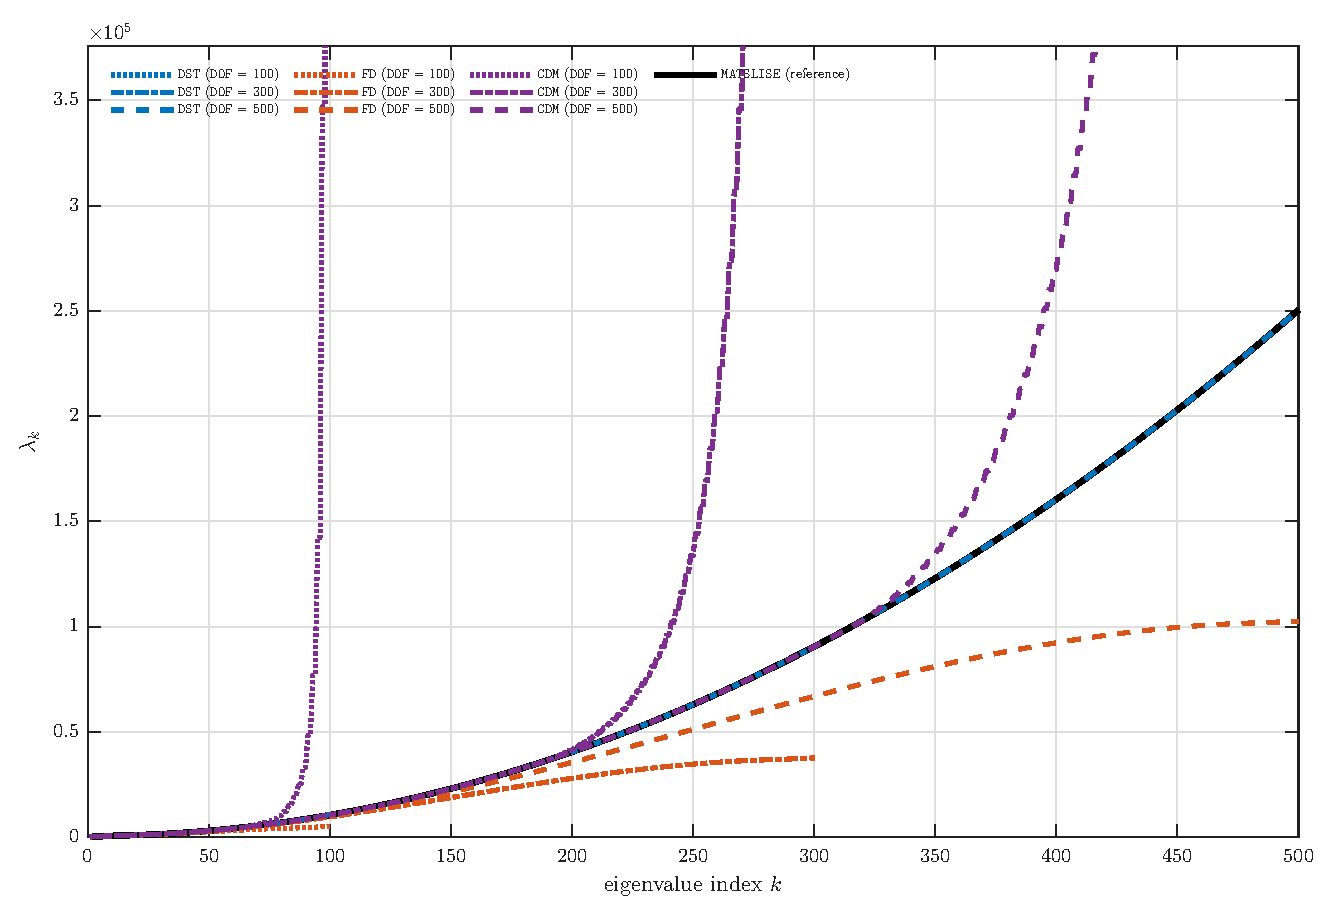
\includegraphics[width=0.8\textwidth]{coffey_evans_dof_sweep_colour_a}}
  \\
  \subfloat[\texttt{MBCDM}, \texttt{Numerov}, \texttt{Numerov+AC} and \texttt{LGCC}.\label{fig:dof_sweep_coffey_evans_colour_b}]{%
    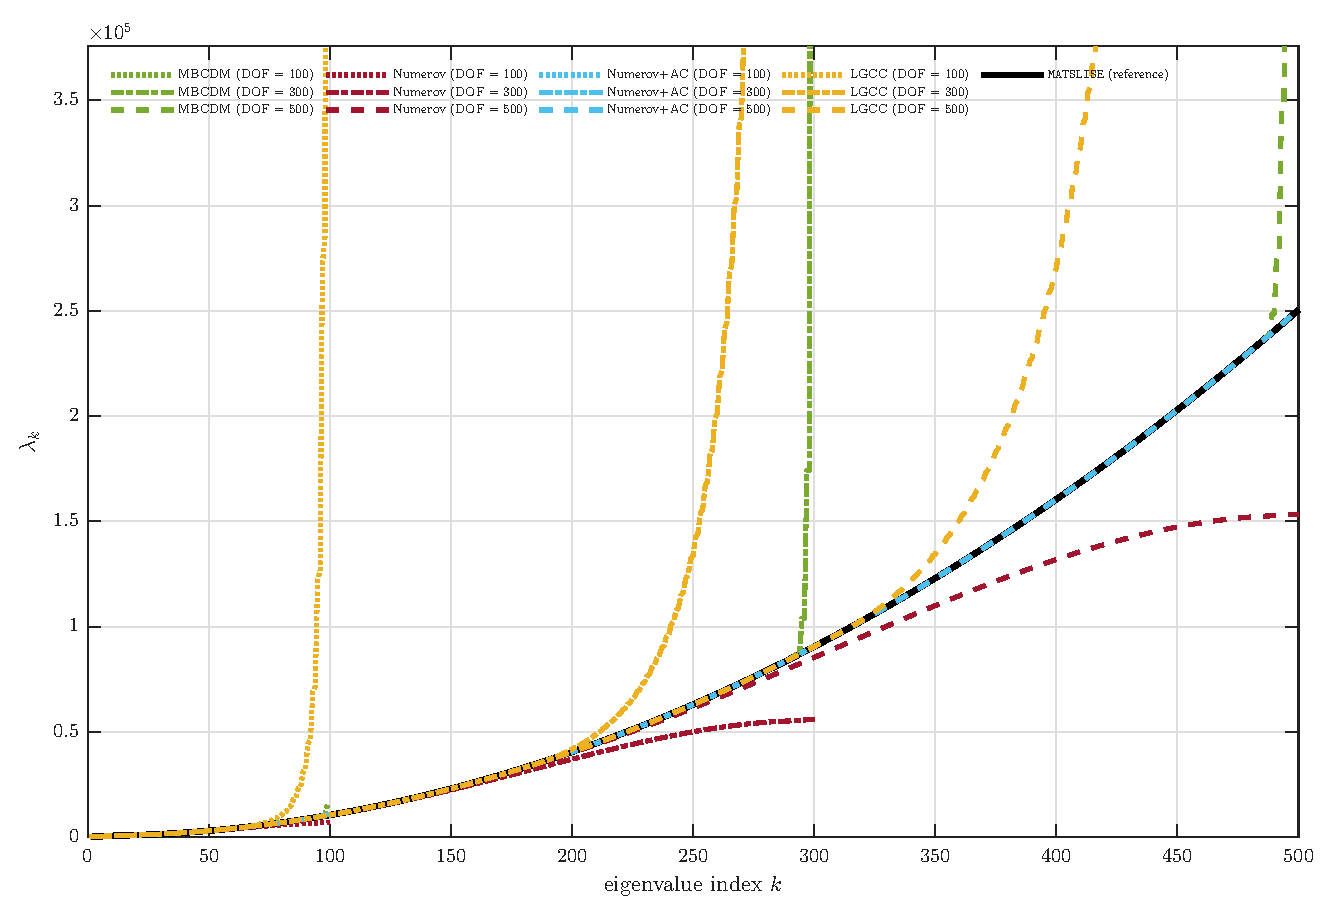
\includegraphics[width=0.8\textwidth]{coffey_evans_dof_sweep_colour_b}}
  \caption{Coffey--Evans problem. Comparison of the reference eigenvalues computed with \texttt{MATSLISE} and the eigenvalues computed using various discretisations at several numbers of degrees of freedom (\texttt{DOF}) each; \texttt{DST} -- discrete sine transform method, \texttt{FD} -- finite differences method, \texttt{CDM} -- Chebyshev differentiation matrix method, \texttt{MBCDM} -- mapped barycentric Chebyshev differentiation matrix method, \texttt{Numerov} -- Numerov method, \texttt{Numerov+AC} -- Numerov method with the asymptotic correction, \texttt{LGCC} -- Legendre--Galerkin method. Both panels repeat the reference.}
  \label{fig:dof_sweep_coffey_evans_colour}
\end{figure}
